\chapter{Background}
\label{chapter:background}
\section{Option Types}
Before completely focusing on the mechanics of options, what influences their prices and how we can predict their behavior, we should begin by clearly defining the main option types, their characteristics, as well as their payoff functions. We will not only approach the two main types of options - European and American - but also other less common types, commonly referred to as Exotic options, such as Asian, Barrier and Binary options.



\subsection{European Options}
\emph{European options} are the most traded type of option in the OTC market~\cite{InvEuro}. They are not only extremely useful to investors, but also very simple to study and comparatively easy to price. For all these reasons, they have been the subject of much research and are deeply understood. Furthermore, because of their high availability, they are very useful in model calibration and validation.


As stated before, call and put European options enable their buyers to respectively buy and sell the underlying asset \emph{at the maturity} for the fixed strike price.

To understand the payoff function of such contracts, we'll use an example. In the case of a European call option, if at the maturity the market price of its underlying asset is greater than the strike, investors can exercise the option and buy the asset for the fixed lower strike price. They can then immediately go to the market and sell the asset for its higher value. Thus, in this case, the payoff of the option would be the difference between the asset's price and the option's strike price. On the other hand, if at the maturity the price of the asset decreases past the strike, the investor should let the option expire, since the asset is available in the market for a lower price. In this case, the payoff would be zero.
The same reasoning can be made for European put type options, such that the payoff function of both option types can then be deduced as
\begin{equation}\label{callput}
\begin{split}
&\text{Payoff}_{Euro,\ call}(K,T)=\max\left(S(T)-K,0\right);\\
&\text{Payoff}_{Euro,\ put}(K,T)=\max\left(K-S(T),0\right),
\end{split}
\end{equation}
\noindent where $K$ is the option's strike price and $S(T)$ is the asset's price, $S(t)$, at the maturity, $T$. These functions are represented in \autoref{fig:Payoff}.

\begin{figure}[!htb]
    \centering
      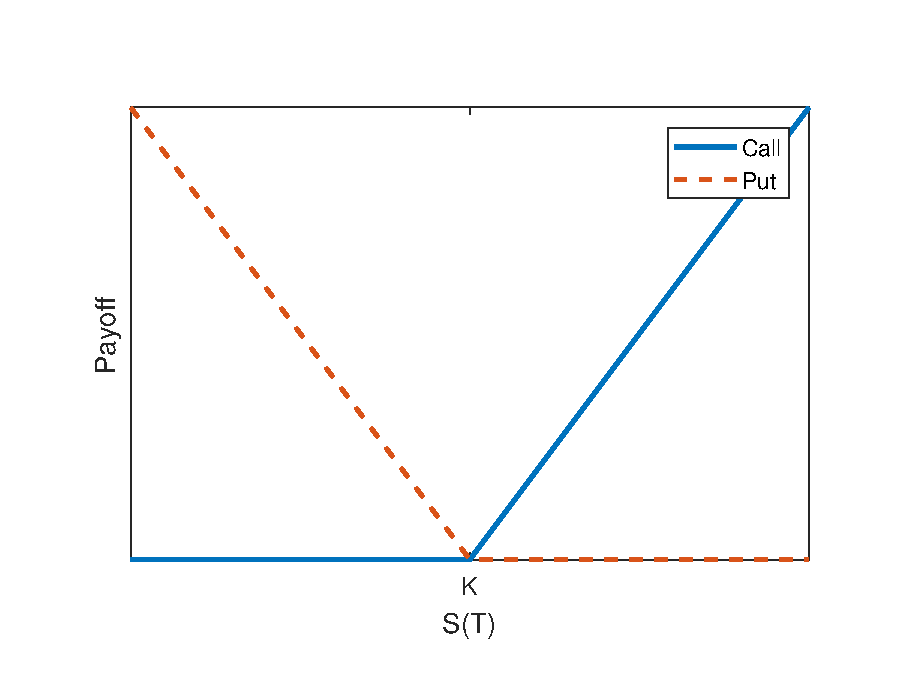
\includegraphics[width=.65\columnwidth]{Payoff.eps}
      \caption[Payoff functions of European call and put options]{Payoff functions of European \emph{call} and \emph{put options}.}\label{fig:Payoff}
    \end{figure}
    



\subsection{American Options}
\emph{American options} are more complex than European and thus harder to price. While European options dominate the OTC market, their American counterparts are the most traded type of option in exchanges~\cite{InvAmer}. Because of their great importance, many models have been developed to find the prices of these options~\cite{Longstaff}.

American options grant the right to buy/sell (call/put) the underlying asset at any point in time \emph{until the maturity date}. Following the logic used in the previous example to find the payoff functions of European calls and puts, we can deduce their American counterparts as
\begin{equation}
\begin{split}
&\text{Payoff}_{Amer,\ call}(K,t^*)=\max\left(S(t^*)-K,0\right);\\
&\text{Payoff}_{Amer,\ put}(K,t^*)=\max\left(K-S(t^*),0\right),
\end{split}
\end{equation}
\noindent where we now define $t^*$ (with $0\leq t^*\leq T$) as the exercise date.

It should be obvious that the price of American options will always be greater or equal to the prices of similar European options. The reason behind this is the fact that, with European contracts our exercise decision is restricted to a single day, whereas with American options we have several other opportunities to make this choice.


\subsection{Exotic Options}
While European and American options are, by far, the most traded types, \emph{Exotic options} should not be neglected. Not only does there exist a great number of Exotic option types, but these are also highly customizable, making this type of derivatives very useful for unconventional investment strategies. Due to their high complexity, these options are only traded in the OTC market, and not in exchanges~\cite{InvExotic}. We will explore three of the most common types of Exotic options, though many others exist.

\subsubsection{Asian Options}
An \emph{Asian} option is an Exotic contract whose payoff depends on the \emph{average value} of an underlying asset. This averaging procedure makes this type of derivative more stable than their European/American equivalents - e.g. if, at the last day of trading, an extreme market event occurs, affecting the price of the underlying asset, an European or American option might suffer radical changes to its value (either beneficial or detrimental), whereas the value of an Asian option should be much less affected by such sudden movements.

The payoff function of this type of contracts is given by
\begin{equation}\label{asian}
\begin{split}
&\text{Payoff}_{Asian,\ call}(K,T)=\max\left(A(S,T)-K,0\right);\\
&\text{Payoff}_{Asian,\ put}(K,T)=\max\left(K-A(S,T),0\right),
\end{split}
\end{equation}
\noindent with $A(S,T)$ corresponding to the arithmetic average of the asset's prices until the maturity,
\begin{equation}\label{avg}
A(S,T)=\frac{1}{T}\int_0^TS(t)dt.
\end{equation}

Other types of Asian option exist: some contracts have a floating strike (i.e. instead of the fixed strike, $K$, the strike is assumed as the average, $A(S,T)$, instead), and others use different types of averaging mechanisms, such as the geometric average. Despite this, we will assume that all Asian options follow the properties described in eqs.\eqref{asian} and \eqref{avg}.


\subsubsection{Barrier Options}
A \emph{Barrier option} behaves similarly to a European option with the difference that it only becomes active (or void) if the value of its underlying asset reaches a particular value, called the \emph{barrier level}, $B$, at any point in time until the option's maturity.

There are four main types of Barrier option:
\begin{itemize}
\item \emph{up-and-out}: the asset's price starts below the barrier (i.e. $S(0)<B$). If it increases past this threshold, the option becomes \emph{worthless};
\item \emph{down-and-out}: the asset's price starts above the barrier (i.e. $S(0)>B$). If it decreases past this threshold, the option becomes \emph{worthless};
\item \emph{up-and-in}: the asset's price starts below the barrier (i.e. $S(0)<B$). Only if it increases past this threshold does the option become \emph{active};
\item \emph{down-and-in}: the asset's price starts above the barrier (i.e. $S(0)>B$). Only if it decreases past this threshold does the option become \emph{active}.
\end{itemize}

Because all of the previously described Barrier option types are handled similarly, we can easily adapt the models from one type to another. Thus, for simplicity, we will henceforth assume that all Barrier options are of the up-and-in type.

Using the up-and-in Barrier option type as an example, if the asset price, $S(t)$, remains below the barrier level $B$ throughout the whole option duration, even if at the maturity the asset's value is higher than the strike price, the option's payoff would nonetheless be zero. On the contrary, if this threshold was surpassed at any point in this period, the option's payoff would be similar to that of its European equivalent.


The payoff function of this type of option is given by
\begin{equation}
\begin{split}
&\text{Payoff}_{Barr,\ call}(K,T)=\begin{cases} 
      \max\left(S(T)-K,0\right), & \mathrm{if}\ \ \exists\,t<T\,:\,S(t)>B\\
      0, & \mathrm{otherwise}
   \end{cases};\\
&\text{Payoff}_{Barr,\ put}(K,T)=\begin{cases} 
      \max\left(K-S(T),0\right), & \mathrm{if}\ \ \exists\,t<T\,:\,S(t)>B\\
      0, & \mathrm{otherwise}
   \end{cases}.
\end{split}
\end{equation}



   
   
\subsubsection{Binary Options}
As the name implies, a \emph{Binary option} is a contract that has one of two outcomes: if at the maturity date the asset price is above/below the strike (call/put), the investor receives a fixed amount of money, $C$. If this event does not occur, the investor receives nothing.

The main difference between a Binary and an European option is the fact that the payoff of a Binary contract is fixed, regardless of the asset price at the maturity, which is not true for European options.

The payoff of this function is, thus,
\begin{equation}\label{binary}
\begin{split}
&\text{Payoff}_{Bin,\ call}(K,T)=\begin{cases} 
      C, & \mathrm{if}\ \ S(T)>K\\
      0, & \mathrm{otherwise}
   \end{cases};\\
&\text{Payoff}_{Bin,\ put}(K,T)=\begin{cases} 
      C, & \mathrm{if}\ \ S(T)<K\\
      0, & \mathrm{otherwise}
   \end{cases}.
\end{split}
\end{equation}


Though all the option types described before are used by banks and investors everyday, we will mainly focus on European options, for the reasons mentioned. One further reason for this choice is the fact that the data available for model calibration and validation pertains only to this option type.
The remaining types will nonetheless be implemented and studied, though no benchmark will be used to verify the models' validity in these cases.


\section{Option Prices and Payoffs}
It is important to emphasize the difference between an option's payoff and its profit for investors. Because options grant the right to buy/sell some asset, no investors would exercise an option if this action was disadvantageous to them (i.e. negative payoff value). Thus, the payoff of an option is always positive (it can also, obviously, be zero). This might sound like an arbitrage possibility (i.e. the chance of making profit without risk - which is illegal), but in reality options have a price that investors have to pay in order to acquire them. This means that even if the option's payoff is positive, if this value is lower than the price an investor paid to buy the option, that investor will actually lose money. The profit of an option is thus the difference between its payoff and its price, which can be negative.
With this concept in mind, we can price options by setting their expected profit to be the same as a risk-neutral investment, (e.g. bank deposit). The price of an option can thus be deduced as it's expected future payoff, discounted back to the present
\begin{equation}
\text{Price}(K,t^*)=e^{-rt^*}\mathbb{E}\left[\text{Payoff}(K,t^*)\right],
\end{equation}
\noindent where $t^*$ denotes the time at which the option is exercised and $r$ corresponds to the risk-free interest rate, which we will approach in Section \ref{section:Black-Scholes Formulae}.



As an example, we now present the price functions of European call and put options.
With eqs.\eqref{callput} in mind, it should be clear that the value of these two types of contracts is given by
\begin{equation}\label{callprice}
\begin{split}
&C(K,T)_{Euro}=e^{-rT}\mathbb{E}\left[\max\left(S(T)-K,0\right)\right]=e^{-rT}\mathbb{E}\left[\left(S(T)-K\right)\mathbbm{1}_{\left\{S(T)>K\right\}}\right];\\
&P(K,T)_{Euro}=e^{-rT}\mathbb{E}\left[\max\left(K-S(T),0\right)\right]=e^{-rT}\mathbb{E}\left[\left(K-S(T)\right)\mathbbm{1}_{\left\{S(T)<K\right\}}\right],
\end{split}
\end{equation}
\noindent with $C(K,T)$ and $P(K,T)$ being the values of European call and put options, respectively, and $\mathbb{E}[\cdot]$, $\mathbbm{1}_{\{\cdot\}}$ corresponding to the expected value and indicator functions, respectively.

When selling or buying options, investment banks add some premium to this zero-profit price, to account for the risk taken. Though this premium is important to define, it is besides the scope of this work and will not be considered here.
    
\section{Black-Scholes Formulae}
\label{section:Black-Scholes Formulae}
Due to their high importance, options have been studied in great detail in the past.
Probably the most important result in this field came from Fischer Black, Myron Scholes and Robert Merton, who developed a mathematical model to price European options - the famous Black-Scholes (BS) model~\cite{Scholes} - still in use in present days~\cite{Wilmott3}.

This model states that the price of an European call or put option follows the partial differential equation (PDE)

\begin{equation}\label{BS2}
\pdv{V}{t}+\frac{1}{2}\sigma^2S^2\pdv{^2V}{S^2}+rS\pdv{V}{S}-rV=0,
\end{equation}

\noindent where $V$ is the price of the option, $S$ is the price of the underlying (risky) asset, $r$ is the risk-free interest rate and $\sigma$ is the stock price volatility.
The underlying asset is commonly referred to as \emph{stock}, so these terms will be used interchangeably in the following sections.


The risk-free interest rate, $r$, is the interest an investor would receive from any risk-free investment (e.g. treasury bills). No investor should ever invest in risky products whose expected return is lower than this interest (e.g. the lottery), since there's the alternative of obtaining a higher (expected) payoff without the disadvantage of taking risks. In general, this rate changes slightly with time and is unknown, but Black \textit{et al.}, in their original model (eq.\eqref{BS2}), assumed that it remains constant throughout the option's duration and that it is known. Some authors have suggested solutions to deal with this shortcoming, providing models to replicate the behavior of interest rates~\cite{HJM}, but because option prices do not significantly depend on this value~\cite{Wilmott3}, in the remainder of this thesis we shall make the same assumptions as Black \textit{et al.} and set this rate to some constant.

As for the stock price volatility, $\sigma$, since we will explore it to great extent in the next sections, suffice it to say that it is a measure of the future stock price movement's uncertainty.

Some companies decide to grant their shareholders a part of the profits generated, known as \emph{dividends}. This action decreases the company's total assets, which decreases the value of stocks, changing option prices. Because this occurrence is based on human decisions, it is extremely hard to model. Furthermore, Black \textit{et al.} assumed in their models that no dividends were paid throughout the option's duration. For both these reasons, we will henceforth set dividend payment to zero.


One other important assumption of the BS model is that stock prices follow a stochastic process, known as Geometric Brownian Motion, which can be defined as
\begin{equation}\label{GBM}
dS(t)=rS(t)dt+\sigma S(t)dW(t),
\end{equation}
\noindent with $\{W(t),\ t>0\}$ defining a one-dimensional Brownian motion and where we define $S_0=S(0)$ as the stock price at time $t=0$. An example of such processes is represented in \autoref{fig:GBM}.
\begin{figure}[!htb]
    \centering
      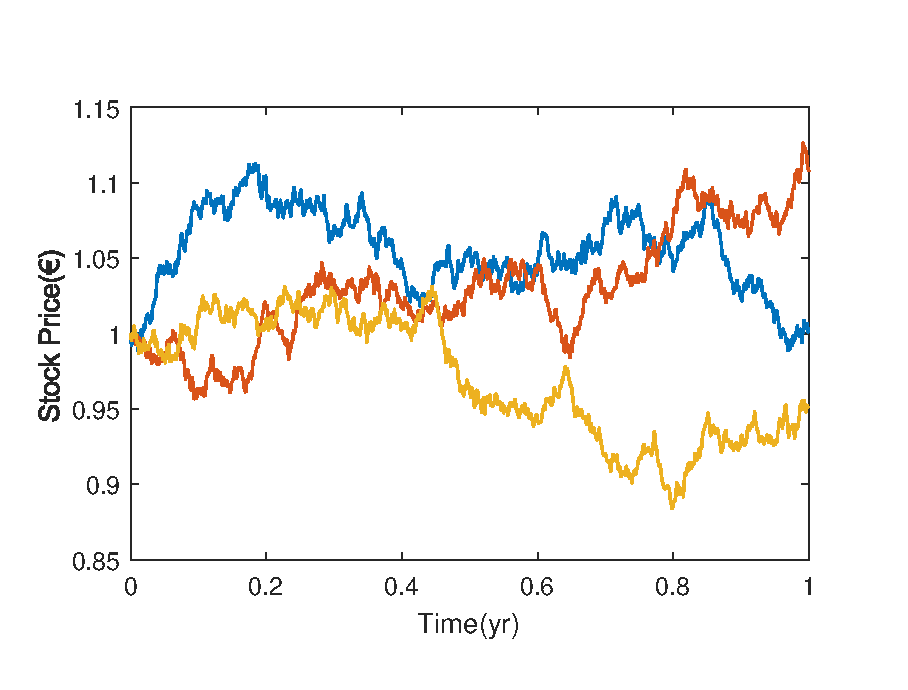
\includegraphics[width=.65\columnwidth]{GBM.eps}
      \caption[Example of Geometric Brownian Motion processes]{Example of three Geometric Brownian Motion processes with maturity $T=\SI{1}{\year}$, interest rate $r=\SI{0.01}{\per\year}$, volatility $\sigma=\SI{0.1}{\year\tothe{-1/2}}$ and initial stock price $S_0=\SI{1}{\EUR}$.}\label{fig:GBM}
    \end{figure}

With this result, pricing options is fairly straightforward - we simply need to solve the PDE in eq.\eqref{BS2} as we would for the diffusion equation's initial value problem~\cite{Dilao}.
The results published originally by Black \textit{et al.} state that, at time $t$, call and put options can be valued as
\begin{equation}\label{callputBS}
\begin{split}
&C(S(t),t)=N(d_1)S(t)-N(d_2)Ke^{-r(T-t)};\\
&P(S(t),t)=-N(-d_1)S(t)+N(-d_2)Ke^{-r(T-t)},
\end{split}
\end{equation}
\noindent where $N(\cdot)$ is the cumulative distribution function of the standard normal distribution and where $d_1$, $d_2$ are given by
\begin{equation}\label{d1d2}
\begin{split}
&d_1=\frac{1}{\sigma\sqrt{T-t}}\left[\ln\left(\frac{S_t}{K}\right)+\left(r+\frac{\sigma^2}{2}\right)(T - t)\right];\\
&d_2=d_1-\sigma\sqrt{T-t}.\\
\end{split}
\end{equation}



From eq.\eqref{callputBS} we can derive the relationship between $C(S,t)$ and $P(S,t)$, known as the \emph{put-call parity}
\begin{equation}
C(S(t),t)=S(t)-Ke^{-r(T-t)}+P(S(t),t).
\end{equation}
\noindent Because of this duality, we can always easily obtain the prices of put options from the prices of call options with the same underlying asset, maturity and strike. For this reason, some of the results presented in later sections only apply to call options, though we can just as easily find their put option equivalent.


\section{Volatility}
\label{section:volatility}
As mentioned, volatility is a measure of the uncertainty of future stock price movements. In other words, a higher volatility will lead to greater future fluctuations in the stock price, whereas a stock with lower volatility is more stable. This phenomenon is exemplified in \autoref{fig:VarVol}, where we can see the greater fluctuations of the high-volatility process (red) compared to the much smaller variations of the low-volatility process (orange).
\begin{figure}[!htb]
    \centering
      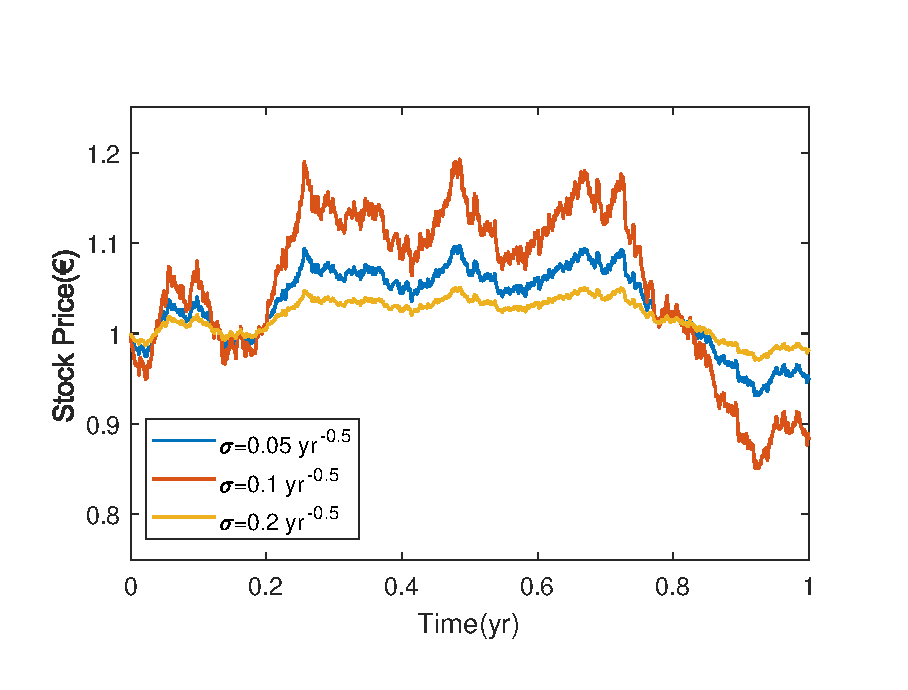
\includegraphics[width=.65\columnwidth]{VarVol.eps}
      \caption[Example of three identical GBM processes with different volatilities]{Example of three identical GBM processes with maturity $T=\SI{1}{\year}$, interest rate $r=\SI{0.01}{\per\year}$ and initial stock price $S_0=\SI{1}{\EUR}$. The volatilities are $\sigma=\SI{0.05}{\year\tothe{-1/2}}$, $\sigma=\SI{0.1}{\year\tothe{-1/2}}$ and $\sigma=\SI{0.2}{\year\tothe{-1/2}}$ for the orange, blue and red plot lines represented, respectively. To emphasize this effect, the underlying Brownian Motion $W(t)$ used to generate all three paths was the same.}\label{fig:VarVol}
    \end{figure}

Of all the parameters in the BS formula (eq.\eqref{BS2}), volatility is the only one we can't easily measure from market data.
Furthermore, unlike the interest rate, volatility has a great impact on the behavior of stock prices and, consequently, on the price of options~\cite{Wilmott3}.
These two factors make volatility one of the most important subjects in all of mathematical finance and thus the focus of much research.



It should be noted that there are several types of volatility, depending on what is being measured. Some of these types will now be introduced and studied.

\subsection{Implied Volatility}
\label{section:impliedvolatility}
\emph{Implied volatility} can be described as the value of stock price volatility that, when input into the BS pricer in eq.\eqref{callputBS}, outputs a value equal to the market price of a given option.
In other words, it would be the stock price volatility that the seller/buyer of the option used when pricing it (assuming the BS model was used).

Because eq.\eqref{callputBS} is not invertible, we need to use some numerical procedure (e.g. Newton's method) to find the value of implied volatility that matches the market and model prices, i.e. we must find, numerically, the solution to the equation
\begin{equation}\label{impvolform}
C(\sigma_{imp},S(t),t)-\overline{C}=0,
\end{equation}
\noindent where $C(\sigma_{imp},\cdot)$ corresponds to the result of eq.\eqref{callputBS} using $\sigma_{imp}$ as (implied) volatility and $\overline{C}$ the price of the option observed in the market.

Because eq.\eqref{callputBS} is monotonic w.r.t. the volatility, we can obtain the implied volatility of an option from its price and vice versa. This duality is so fundamental that investors often disclose options by providing their implied volatility instead of their price~\cite{Wilmott}.

One important property of implied volatility is that, in the real-world, it depends on the strike price and the maturity. This should not occur in the "Black-Scholes world". Because the volatility is a property of the stock, if investors really used the the BS model to price their options, two options with the same underlying stock should have the same implied volatility, regardless of their strike prices or maturities (i.e. the same stock can't have two different volatilities at the same time).
However, when observing real market data, this is in fact what is observed.
The implied volatilities' dependence on the strike price can take one of two forms, known as \emph{smile} and \emph{skew}.
An implied volatility smile presents higher volatilities for options with strikes farther from the current stock price (i.e. the shape of a smile). A skew, on the other hand, only presents higher volatilities in one of these directions (i.e. only for strikes either greater or smaller than the current stock price). Both phenomena are represented in \autoref{fig:smileskew}.
\begin{figure}[!htb]
  \begin{subfigmatrix}{2}
    \subfigure[Smile]{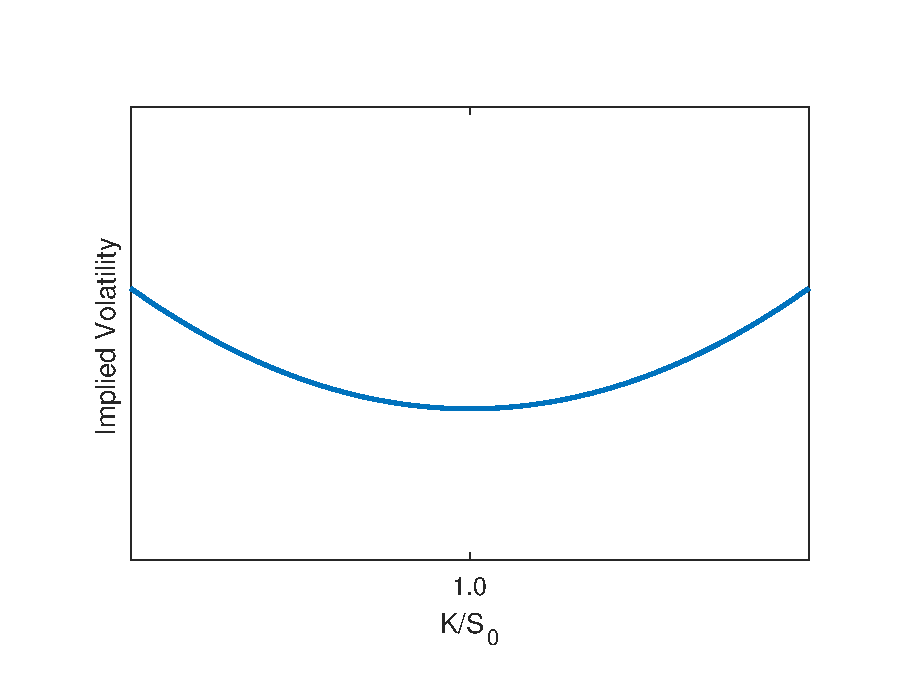
\includegraphics[width=0.49\linewidth]{Smile.eps}}
    \subfigure[Skew]{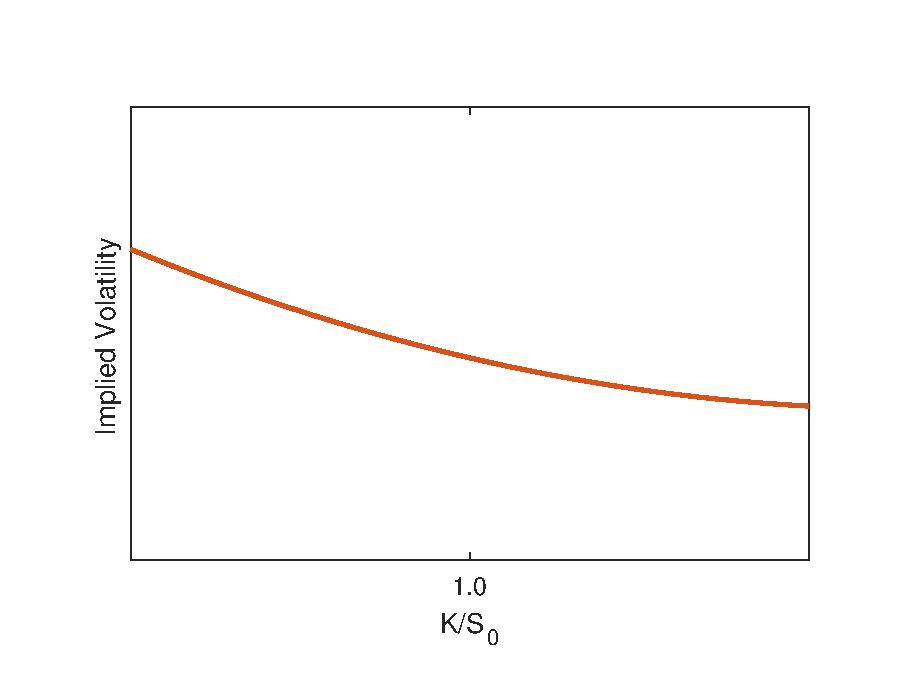
\includegraphics[width=0.49\linewidth]{Skew.eps}}
  \end{subfigmatrix}
  \caption[Representation of the implied volatility smile and skew functions.]{Representation of the implied volatility smile (left) and skew (right) functions.}
  \label{fig:smileskew}
\end{figure}


Because of their higher implied volatility, we can conclude that options with strikes different from the current stock price are \emph{overpriced}.
The reason behind this odd market behavior is related to the simple demand-supply rule~\cite{Wilmott3}. On the one hand, some investors are risk-averse and want to hedge their losses in case of a market crash (as explained in subsection \ref{subsection:why options are important}). They don't mind paying a higher price for an option if this means they would be relatively safe from potentially devastating market crashes. For this reason, the prices of call options with lower strikes increase, driving their implied volatility up. On the other hand, other investors are risk-seekers and want to take advantage of possible sudden price movements, buying the stocks for the lower strike prices. They don't mind paying higher prices for the chance of earning high profits and this drives the prices of high strike call options (and, consequently, their implied volatility) up. This fear-greed duality gives rise to the observed volatility smile. 
In the case of the volatility skew, only one of the two fenomena described occurs.




The presence of a smile instead of a skew, and vice-versa, is determined by the type of product serving as underlying asset. For example, Forex market options usually exhibit volatility smiles whereas index and commodities options usually present a volatility skew.

The dependence of the implied volatility on the maturity date is more complex, but in general it decreases with $T$.

It can also be shown that the implied volatility is the same for calls and puts~\cite{Hull}, though the causes of the volatility smile/skew for put options are the opposite of the ones described before, for calls.

\subsection{Local Volatility}
\label{subsection:localvolatility}
In their original work, Black \textit{et al.} assumed that volatility is constant throughout the whole option duration. From market data, it can be clearly seen that this is not the case~\cite{DJIA}. There may be times where new information reaches the market  (e.g. the results of an election) and trading increases, driving volatility up. It is equally true that shortly before this information is known, trading may stall, and volatilities go down. 

The BS model is therefore clearly incapable of completely grasping real-world trading. We should use a model where volatility is dynamic, measuring the uncertainty on the stock price movement at any point in time.
However, as we saw in subsection \ref{section:impliedvolatility}, the market's view of volatility also depends on the strike price.
The volatility should therefore be a function of both time and stock price: $\sigma(S,t)$. We call this model \emph{local volatility} and the geometric Brownian motion from eq. \ref{GBM} is transformed into
\begin{equation}\label{GBM2}
dS(t)=rS(t)dt+\sigma(S,t)S(t)dW(t),
\end{equation}
\noindent where $\sigma(S,t)$ is some function of $S$ and $t$.


We should note that finding the local volatility function is unnecessary when pricing European options - we can simply find the implied volatility of the option we're pricing from the data of similar options in the market and then use eq.\eqref{callputBS}, assuming a constant volatility, to find the price of the European option.
However, for other contracts, such as American, Asian or Barrier options (among others), where the option's value depends on the intermediate stock prices, it is indeed crucial to appropriately model the volatility.

Because we can't directly measure the local volatility of a stock from market data, we need some models to find it. One of the most used of these is known as Dupire's formula.

\subsubsection{Dupire's Formula}
\label{subsubsection:Dupire}
One of the most famous results in the modelling of the local volatility function was obtained by Dupire~\cite{Dupire}. In his article, this author derives a theoretical formula for $\sigma(S,t)$, given by
\begin{equation}\label{dupire}
\sigma(S,t)=\sqrt{\frac{\displaystyle\pdv{C}{T}+rS\pdv{C}{K}}{\displaystyle\frac{1}{2}S^2\pdv{^2C}{K^2}}},
\end{equation}
\noindent where $C=C(K,T)$ is the price of an European call option with strike price $K$ and maturity $T$. All the derivatives are evaluated at $K=S$ and $T=t$.




\begin{proof}

We begin by assuming that the stock price $S$ follows a dynamic transition probability density function $p(S(t),t,S'(t'),t')$. In other words, by integrating this density function we would obtain the probability of the stock price reaching a price $S'$ at a time $t'$ having started at $S$ at time $t$.

The present value of a call option, $C(S,t,K,T)$, can be deduced as its expected future payoff, discounted backwards in time, which results in
\begin{equation}
\begin{split}\label{deriv0}
C(K,T)=e^{-r(T-t)}\mathbb{E}\left[\max\left(S'-K,0\right)\right]&=e^{-r(T-t)}\int_0^\infty\max\left(S'-K,0\right)p(S,t,S',T)dS'\\
&=e^{-r(T-t)}\int_K^\infty(S'-K)p(S,t,S',T)dS'.
\end{split}
\end{equation}
Taking the first derivative of this result with respect to the strike price $K$, we obtain
\begin{equation}
\pdv{C}{K}=-e^{-r(T-t)}\int_K^\infty p(S,t,S',T)dS'.
\end{equation}
The second derivative results in
\begin{equation}
\pdv{^2C}{K^2}=e^{-r(T-t)}p(S,t,S',T).
\end{equation}

Due to its stochastic nature, the transition probability density function follows the Fokker-Planck equation, given by
\begin{equation}\label{FokkerPlanck}
\pdv{p}{T}=\frac{1}{2}\sigma^2\pdv{^2(S^2p)}{S^2}-r\pdv{(Sp)}{S}.
\end{equation}
\noindent with $\sigma$ denoting our (still unknown) function of $S$ and $t$, evaluated at $t=T$.

From eq. \ref{deriv0} we can easily derive
\begin{equation}
\pdv{C}{T}=-rC+e^{-r(T-t)}\int_K^\infty(S'-K)\pdv{p}{T}dS'.
\end{equation}
Using eq. \ref{FokkerPlanck}, we can transform this relation into
\begin{equation}
\pdv{C}{T}=-rC+e^{-r(T-t)}\int_K^\infty(S'-K)\left(\frac{1}{2}\sigma^2\pdv{^2(S'^2p)}{S'^2}-r\pdv{(S'p)}{S'}\right)dS'.
\end{equation}
Integrating twice by parts and collecting all terms, we get
\begin{equation}
\pdv{C}{T}=\frac{1}{2}\sigma^2K^2\pdv{^2C}{K^2}-rK\pdv{C}{K}.
\end{equation}
Rearranging all terms, we are left with
\begin{equation}
\sigma(K,T)=\sqrt{\frac{\displaystyle\pdv{C}{T}+rK\pdv{C}{K}}{\displaystyle\frac{1}{2}K^2\pdv{^2C}{K^2}}},
\end{equation}
\noindent from which we can easily derive Dupire's formula, as shown in eq.\eqref{dupire}, using a simple variable change, i.e. $\sigma(K,T)\implies \sigma(S,t)$, which gives
\begin{equation}
\sigma(S,t)=\sqrt{\frac{\displaystyle\pdv{C}{T}+rS\pdv{C}{K}}{\displaystyle\frac{1}{2}S^2\pdv{^2C}{K^2}}}.
\end{equation}
\end{proof}

As can be seen, we need to differentiate the option prices with respect to their strikes and maturities. To achieve this, we need first to gather, from the market, a large number of prices for options with different maturities and strikes. We then implement some interpolation on these values to obtain an option price surface (with $K$ and $T$ as variables). Finally, we calculate the gradients of this interpolated surface and input them into eq.\eqref{dupire} to obtain the local volatility surface.
We can then sample the local volatility at each time step of our simulation.


Even before implementation, four potential sources of error can be found:
\begin{itemize}
\item First, it should be noted that markets only trade options with very specific maturities (e.g. 1, 2, 4 and 6-months maturity). For this reason, our data will be extremely sparse w.r.t. maturity and the interpolation generated may not correspond to reality.
\item Furthermore, it can be shown that, for strikes much greater or much smaller than the current stock price, the option price's dependence on the strike is approximately linear. The second derivative in these regions would therefore be very close to zero. Because this second derivative is in the denominator of eq.\eqref{dupire}, the obtained volatilities may explode for very large or very small strikes.
\item There is also the problem of noise. Because we are interpolating very sparse data, even small fluctuations in the option market price may cause great variations in the option price interpolation. This can be specially problematic in regions where the second derivative is small, because, as discussed, the volatility is very sensitive to this value.
\item Finally, some problems arise from the market itself. While most investors use some theoretical basis in their trades, the market is still governed by the demand-supply rule. If too many investors want to buy the option and few want to sell it, the option price will increase, even if it means that the option will be overpriced, and vice versa. Furthermore, the market is not very liquid for options with very large maturities or very large/small strikes (i.e. almost no trade occurs for these options) which causes the option prices to not truly follow the market's perception of future price movements.
\end{itemize}
All these problems must be taken into account when applying Dupire's model.




Fortunately, Dupire also developed an alternative local-volatility formula based on the implied volatility surface instead of the option price's, as seen in eq.\ref{dupire}.
The relation obtained is
\begin{equation}\label{dupire2}
\sigma(S,t)=\sqrt{\frac{\displaystyle\sigma_{imp}^2+2t\sigma_{imp}\pdv{\sigma_{imp}}{T}+2rSt\sigma_{imp}\pdv{\sigma_{imp}}{K}}{\displaystyle\left(1+Sd_1\sqrt{t}\pdv{\sigma_{imp}}{K}\right)^2+S^2t\sigma_{imp}\left(\pdv{^2\sigma_{imp}}{K^2}-d_1\left(\pdv{\sigma_{imp}}{K}\right)^2\sqrt{t}\right)}},
\end{equation}
\noindent where $d_1$ is given by
\begin{equation}
d_1=\frac{\log(S_0/S)+\left(r+\frac{1}{2}\sigma_{imp}^2\right)t}{\sigma_{imp}\sqrt{t}},
\end{equation}
\noindent with $S_0$ being the stock price at $t=0$. We define $\sigma_{imp}=\sigma_{imp}(K,T)$ as the interpolated surface of the implied volatilities evaluated at time $T$, and price $K$. All derivatives are also evaluated at $K=S$ and $T=t$. This formula can be obtained from eq.\eqref{dupire} by applying the transformation from call prices to implied volatilities.

Because some of the shortcomings described for eq.\eqref{dupire} do not apply to eq.\eqref{dupire2}, and because the latter is more stable than the former~\cite{Wilmott3}, this new equation will be adopted in the implementation.


Two other problems can be identified in Dupire's local volatility assumption, however.
First, it can be shown that if the local volatility surface truly matched reality, it should remain unchanged, i.e. the local volatility surface measured today and again in one month's time should, in theory, be the same. However, by studying market data, we can see that this is really not the case~\cite{Wilmott3}. We can therefore conclude that the model doesn't completely correspond to reality and for that reason it shouldn't be used blindly.
Furthermore, some authors have also pointed out that the volatility smile obtained from Dupire's local-volatility model doesn't follow real market dynamics~\cite{Hagan}: it can be shown that when the price of the stock either increases or decreases, the volatility smile predicted by Dupire's model shifts in the opposite direction. The minimum of the volatility smile would therefore be offset and no longer correspond to the local stock price. The volatility smile dynamics obtained from the local-volatility model would thus be actually worse than if we assumed a constant volatility.

Despite its problems, Dupire's formula is still very much used in real-world practice and performs surprisingly well, as we will see in later chapters.

\subsection{Stochastic Volatility}
\label{subsection:stochastic volatility}
As stated before, the volatility is not constant, is not observable and is not predictable, despite our attempts to model it. This seems to indicate that volatility is itself also a stochastic process. Some research has been done into this hypothesis, and many models have been developed to replicate real-world volatilities.

As before, we assume that the stock price follows a geometric Brownian motion
\begin{equation}\label{stochvol}
dS(t)=rS(t)dt+\sigma(S,t)S(t)dW_1(t),
\end{equation}
\noindent but we further hypothesize that the volatility follows
\begin{equation}
d\sigma(S,t)=p(S,\sigma,t)dt+q(S,\sigma,t)dW_2(t),
\end{equation}
\noindent where $p(S,\sigma,t)$ and $q(S,\sigma,t)$ are some functions of the stock price $S$, time $t$ and of the volatility $\sigma$ itself. We also assume that $W_1$ and $W_2$ are two Brownian motion processes with a correlation of $\rho$, i.e.
\begin{equation}
dW_1dW_2=\rho dt.
\end{equation}
\noindent This correlation factor $\rho$ can be explained by the relationship between prices and volatilities. Usually, when prices decrease, trade goes up and thus rises the volatility. The inverse is true when prices increase. This seems to indicate the existence of a negative correlation between stock prices and volatilities, though positive correlations are also possible.



Choosing the appropriate functions $p(S,\sigma,t)$ and $q(S,\sigma,t)$ is very important since the whole evolution of the stock price depends on them. All stochastic volatility models present a different version of these functions, and each may be more adequate for some types of assets. Furthermore, these functions have some parameters that we have to calibrate in order to best fit our model to market data, as we will see later.

We now present two of the most used stochastic volatility models - \emph{Heston} and \emph{SABR}.



\subsubsection{Heston Model}
\hl{show proof in appendix}

\hl{Feller condition}

One of the most popular stochastic volatility models is known as \emph{Heston model}. It was developed in 1993 by Steven Heston~\cite{Heston} and it states that stock prices satisfy the relations
\begin{equation}
dS=rSdt+\sqrt{\nu}SdW_1,
\end{equation}
\begin{equation}
d\nu=\kappa(\overline{\nu}-\nu)dt+\eta\sqrt{\nu}dW_2,
\end{equation}
\noindent with $\nu$ corresponding to the stock price variance (i.e. $\nu=\sigma^2$) and again where $W_1$ and $W_2$ have a correlation of $\rho$. We furthermore define $\nu_0$ as the initial variance (i.e. variance at time $t=0$). The original model used a drift parameter $\mu$ instead of the risk-free measure drift $r$ presented here, but a measure transformation, using Gisarnov's theorem, can be easily implemented~\cite{Crisostomo}.

The parameters $\kappa$, $\overline{\nu}$ and $\eta$ are, respectively, the mean-reversion rate (i.e. how fast the volatility converges to its mean value), the long-term variance (i.e. the mean value of variance) and the volatility of volatility (i.e. how erratic is the volatility process).



One of the reasons why the Heston model is so popular is the fact that there exists a closed-form solution for the prices of European options priced under this model. This closed form solution is given by
\begin{equation}\label{CH}
\begin{split}
C_{H}(\theta;K,T)&=e^{-rT}\mathbb{E}\left[\left(S(T)-K\right)\mathbbm{1}_{\left\{S(T)>K\right\}}\right]\\
&=e^{-rT}\left(\mathbb{E}\left[S(T)\mathbbm{1}_{\left\{S(T)>K\right\}}\right]-K\mathbb{E}\left[\mathbbm{1}_{\left\{S(T)>K\right\}}\right]\right)\\
&=S(0)P_1-e^{-rT}KP_2,
\end{split}
\end{equation}
\noindent where $C_{H}(\theta;K,T)$ corresponds to the theoretical European call option price under the Heston model, assuming a parameter set $\theta$, strike $K$ and maturity $T$. The variables $P_1$ and $P_2$ are given by
\begin{equation}\label{P1}
P_1=\frac{1}{2}+\frac{1}{\pi}\int_0^\infty\operatorname{Re}\left(\frac{e^{-iu\log K}}{iuS(0)e^{rT}}\phi(\theta;u-i,T)\right)du,
\end{equation}
\begin{equation}\label{P2}
P_2=\frac{1}{2}+\frac{1}{\pi}\int_0^\infty\operatorname{Re}\left(\frac{e^{-iu\log K}}{iu}\phi(\theta;u,T)\right)du,
\end{equation}
\noindent where $i$ is the imaginary unit and $\phi(\theta;u,t)$ is the characteristic function of the logarithm of the stock price process - the characteristic function of a random variable is the Fourier transform of the probability density function of that variable.


It is crucial to find the appropriate characteristic function $\phi(\theta;u,t)$ in order to evaluate the integrals in eqs.\eqref{P1} and \eqref{P2} and with them find the option price with eq.\eqref{CH}. In his original article, Heston derived this very characteristic function~\cite{Heston}. However, some authors showed that it contained discontinuities for large maturities and wasn't easily derivable~\cite{Kahl}, making eq.\eqref{CH} very difficult to evaluate. These shortcomings led some other authors to propose several modified versions of this function~\cite{Rollin,Schoutens}. Most recently, Cui \textit{et al.}~\cite{Cui} presented a characteristic function that not only doesn't have the previously mentioned discontinuities but is also easily derivable, given by
\begin{equation}
\phi(\theta;u,t)=\exp\left\{iu\left(\log S_0+rt\right)-\frac{t\kappa\overline{\nu}\rho iu}{\eta}-\nu_0A+\frac{2\kappa\overline{\nu}}{\eta^2}D\right\},
\end{equation}
\noindent with $A$ and $D$ given by
\begin{equation}
A=\frac{A_1}{A_2},
\end{equation}
\begin{equation}
D=\log C+\frac{(\kappa-C) t}{2}-\log\left(\frac{C+\xi}{2}+\frac{C-\xi}{2}e^{-C t}\right),
\end{equation}
\noindent where we introduce the variables $A_1$, $A_2$, $C$  and $\xi$
\begin{equation}
A_1=(u^2+iu)\sinh\frac{Ct}{2},
\end{equation}
\begin{equation}
A_2=C\cosh\frac{C t}{2}+\xi\sinh\frac{C t}{2},
\end{equation}
\begin{equation}
C=\sqrt{\xi^2+\eta^2(u^2+iu)},
\end{equation}
\begin{equation}
\xi=\kappa-\eta\rho iu.
\end{equation}




With this result we are now able to find the prices of options under the Heston model for a given set of parameters $\theta$. However, we need to find the optimal set of parameters such that the Heston model appropriately replicates market prices. This procedure is called called calibration and will be approached in detail in Chapter \ref{chapter:implementation}.

\iffalse
Calibrating the parameters  $\rho$, $\kappa$, $\overline{\nu}$ and $\eta$ is absolutely critical. A model with badly calibrated parameters would output wrong predictions, rendering it completely useless.
This calibration requires a fair amount of past market data and is by far the most complex and computationally demanding section of this model. We will deal with it in the next section.
\fi





\subsubsection{Static SABR Model}
One other very famous model for stochastic volatility was developed by Hagan \textit{et al.}~\cite{Hagan} and is known as \emph{SABR} - we will henceforth refer to it by \emph{Static SABR}, to distinguish it from the \emph{Dynamic SABR} model that we will see next. SABR stands for "\emph{stochastic-}$\alpha\beta\rho$" and in this model it is assumed that the option prices and volatilities follow~\cite{Geeske}
\begin{equation}\label{dF}
dS=rSdt+e^{-r(T-t)(1-\beta)}\sigma S^\beta dW_1,
\end{equation}
\begin{equation}\label{dsigma}
d\sigma=\nu\sigma dW_2,
\end{equation}
\noindent where we define $\alpha=\sigma(0)$ as the starting volatility and $S_0=S(0)$ as the starting stock price. Finally, as before, the two Brownian motion processes $W_1$ and $W_2$ have a correlation of $\rho$.




In the original article, the authors claim that $\beta$ can be fitted from historical market data, but usually investors choose this value heuristically, depending on the type of assets traded. Typical values used are $\beta=1$ (stochastic lognormal model), used for foreign exchange options, $\beta=0$ (stochastic normal model), typical for interest rate options and $\beta=0.5$ (stochastic CIR model), also common for interest rate options.
We will leave this parameter free upon implementation, assuming no heuristics.

One of the main problems with the static SABR model is the fact that, unlike the Heston model, the stochastic volatility process is not mean-reverting. This shortcoming enables the volatility to evolve unrestrictedly which is problematic - it may become negative, which is clearly absurd, or it may become extremely large, which is troublesome. Labordère~\cite{Labordere} proposed a mean-reverting correction to static SABR, but we will study the original model by Hagan \textit{et al.}, as it is more commonly used.

One of the main reasons why static SABR is so popular is due to its quasi-closed-form solutions that enable us to quickly find the implied volatilities of options priced under this model. With the corrections done by Oblój on Hagan's original formula~\cite{Obloj}, it can be shown that these implied volatilities are given by
\begin{equation}\label{sabr}
\begin{split}
\sigma_{SABR}(K,f,T)\approx&\frac{1}{\displaystyle\left[1+\frac{(1-\beta)^2}{24}\log^2\left(\frac{f}{K}\right)+\frac{(1-\beta)^4}{1920}\log^4\left(\frac{f}{K}\right)\right]}.\left(\frac{\nu\log\left(f/K\right)}{x(z)}\right)\\
&.\left\{1+T\left[\frac{(1-\beta)^2}{24}\frac{\alpha^2}{(Kf)^{1-\beta}}+\frac{1}{4}\frac{\rho\beta\nu\alpha}{(Kf)^{(1-\beta)/2}}+\frac{2-3\rho^2}{24}\nu^2\right]\right\},
\end{split}
\end{equation}
\noindent with $z$ and $x(z)$ given by
\begin{equation}
z=\frac{\nu\left(f^{1-\beta}-K^{1-\beta}\right)}{\alpha(1-\beta)},
\end{equation}
\begin{equation}
x(z)=\log\left\{\frac{\sqrt{1-2\rho z+z^2}+z-\rho}{1-\rho}\right\},
\end{equation}
\noindent where we have used $f=S_0e^{rT}$.

Similarly to the Heston model, we again need to find the set of parameters that minimize the difference between the implied volatilities obtained from the model and those obtained from market data. This calibration procedure will also be studied in Chapter \ref{chapter:implementation}.


\subsubsection{Dynamic SABR Model}
One of the main setbacks of the static SABR model is the fact that it only works for a set of options with the same maturity. The model behaves badly when we try to fit options with different maturities~\cite{Hagan}. 

To solve this problem, Hagan \textit{et al.} suggested a similar model known as \emph{Dynamic SABR}~\cite{Hagan}. It follows the same processes presented in eqs.\eqref{dF} and \eqref{dsigma} but with time-dependent parameters $\rho(t)$ and $\nu(t)$,
\begin{equation}\label{dF2}
dS=rSdt+e^{-r(T-t)(1-\beta)}\sigma S^\beta dW_1,
\end{equation}
\begin{equation}\label{dsigma2}
d\sigma=\nu(t)\sigma dW_2,
\end{equation}
\noindent with the correlation between $W_1$ and $W_2$ now given by $\rho(t)$.

Hagan \textit{et al.} derived again a quasi-closed-form solution for the implied volatilities of options priced under this model. Osajima later simplified this expression using asymptotic expansion~\cite{Osajima}. The resulting formula is given by
\begin{equation}\label{dynsabr}
\sigma_{DynSABR}(K,f,T)=\frac{1}{\omega}\left(1+A_1(T)\log\left(\frac{K}{f}\right)+A_2(T)\log^2\left(\frac{K}{f}\right)+B(T)T\right),
\end{equation}
\noindent where $f=S_0e^{rT}$, $\ \omega=f^{1-\beta}/\alpha\ $ and where $A_1(T)$, $A_2(T)$ and $B(T)$ are given by
\begin{equation}
A_1(T)=\frac{\beta-1}{2}+\frac{\eta_1(T)\omega}{2},
\end{equation}
\begin{equation}
A_2(T)=\frac{(1-\beta)^2}{12}+\frac{1-\beta-\eta_1(T)\omega}{4}+\frac{4\nu_1^2(T)+3(\eta_2^2(T)-3\eta_1^2(T))}{24}\omega^2,
\end{equation}
\begin{equation}
B(T)=\frac{1}{\omega^2}\left(\frac{(1-\beta)^2}{24}+\frac{\omega\beta\eta_1(T)}{4}+\frac{2\nu_2^2(T)-3\eta_2^2(T)}{24}\omega^2\right),
\end{equation}
\noindent with $\nu_1^2(T)$, $\nu_2^2(T)$, $\eta_1(T)$ and $\eta_2^2(T)$ defined as
\begin{equation}\label{nu1}
\nu_1^2(T)=\frac{3}{T^3}\int_0^T(T-t)^2\nu^2(t)dt,
\end{equation}
\begin{equation}
\nu_2^2(T)=\frac{6}{T^3}\int_0^T(T-t)t\nu^2(t)dt,
\end{equation}
\begin{equation}
\eta_1(T)=\frac{2}{T^2}\int_0^T(T-t)\nu(t)\rho(t)dt,
\end{equation}
\begin{equation}\label{eta2}
\eta_2^2(T)=\frac{12}{T^4}\int_0^T\int_0^t\left(\int_0^s\nu(u)\rho(u)du\right)^2dsdt,
\end{equation}
\noindent where $\rho(t)$ and $\nu(t)$ are the functions chosen to model the time dependent parameters.


We now need to empirically choose some appropriate functions for $\rho(t)$ and $\nu(t)$.
We can choose these functions such that the integrals in eqs.\eqref{nu1}-\eqref{eta2} are analytically  solvable, greatly simplifying the calibration of this model.
One classical example~\cite{Fernandez} corresponds to
\begin{equation}\label{rhot}
\rho(t)=\rho_0e^{-at},
\end{equation}
\begin{equation}\label{nut}
\nu(t)=\nu_0e^{-bt},
\end{equation}
\noindent with $\rho_0\in[-1,1]$, $\nu_0>0$, $a>0$ and $b>0$.
In this particular case, $\nu_1^2(T)$, $\nu_2^2(T)$, $\eta_1(T)$ and $\eta_2^2(T)$ can be exactly derived as
\begin{equation}
\nu_1^2(T)=\frac{6\nu_0^2}{(2bT)^3}\left[\left(\frac{(2bT)^2}{2}-2bT+1\right)-e^{-2bT}\right],
\end{equation}
\begin{equation}
\nu_2^2(T)=\frac{12\nu_0^2}{(2bT)^3}\left[e^{-2bT}(1+bT)+bT-1\right],
\end{equation}
\begin{equation}
\eta_1(T)=\frac{2\nu_0\rho_0}{T^2(a+b)^2}\left[(a+b)T+e^{-(a+b)T}-1\right],
\end{equation}
\begin{equation}
\eta_2^2(T)=\frac{3\nu_0^2\rho_0^2}{T^4(a+b)^4}\left[e^{-2(a+b)T}-8e^{-(a+b)T}+(7+2T(a+b)(-3+(a+b)T))\right].
\end{equation}

\hl{should we include also this new more complex model?}

Despite their analytically solvable integrals, these formulas may not be robust enough to appropriately fit large data sets. Other more robust examples are
\begin{equation}\label{rhot2}
\rho(t)=(\rho_0+q_\rho t)e^{-at}+d_\rho,
\end{equation}
\begin{equation}\label{nut2}
\nu(t)=(\nu_0+q_\nu t)e^{-bt}+d_\nu,
\end{equation}
\noindent where we have now introduced new parameters $q_\rho$, $d_\rho$, $q_\nu$ and $d_\nu$.
The main problem with these more robust formulas is the increased number of parameters, which makes the calibration procedure much more complex. Furthermore, the integral in eq.\eqref{eta2} is not analytically solvable, and must be calculated numerically, which further complicates the calibration.

Both examples shown before will be analyzed in later chapters. 
